%author: Simone Notargiacomo, Lorenzo Tavernese, Ibrahim Khalili
%date: 19 Giugno 2008
\documentclass[a4paper,italian,12pt]{beamer}
\usepackage[utf8]{inputenc}
\usepackage[italian,english]{babel}
\usepackage[T1]{fontenc}
\usepackage{beamerthemesplit}
\usepackage{graphicx}
\usepackage{float}

\usepackage{times}
\usepackage{colortbl}

%\usepackage{tikz}
%\usetikzlibrary{arrows}
%\tikzstyle{block}=[draw opacity=0.7,line width=1.4cm]

%\setbeamercolor{sidebar right}{bg=black!15}
%\setbeamercolor{structure}{fg=blue}
%\setbeamercolor{author}{parent=structure}

\usetheme{Antibes}
\useoutertheme{smoothbars}
%\useoutertheme{infolines}
%\usecolortheme{rose}
\useinnertheme{circles}

\title{Ingegneria del Web 07/08}
\institute{Università di Roma Tor Vergata}
\author{Simone Notargiacomo}
%\logo{
\includegraphics[scale=0.1]{etc/tortellalogo.jpg}}
\date{\today}

\begin{document}
	\begin{frame}
		\titlepage
		\begin{figure}[H]
			\begin{center}
				
\includegraphics[scale=0.4]{etc/tortellalogo.jpg}
			\end{center}
		\end{figure}
	\end{frame}

    \section{Sommario}
	    \frame{\tableofcontents}

	\section{Protocollo trasporto}
		\subsection{HTTP}
			\begin{frame}
				\frametitle{Definizione header}
				\begin{itemize}
					\item Utilizzati header protocollo versione "1.1".
					\item Realizzati metodi POST e GET.
					\begin{itemize}
						\item I POST trasferiscono tutti i pacchetti TorTella.
						\item I GET servono per richiedere il trasferimento di file.
					\end{itemize}
				\end{itemize}
				\vspace{2mm}
				\begin{columns}
					\footnotesize{
					\begin{column}{0.5\textwidth}			
						Pacchetto di richiesta:\\
						\texttt{					
							POST * HTTP/1.1\\
							User-Agent: TorTella/0.1\\
							Connection: Keep-Alive\\
							Content-Length: <num>
							...data...
						}
					\end{column}
					\begin{column}{0.5\textwidth}
						Pacchetto di risposta:\\
						\vspace{2mm}
						\texttt{					
							HTTP/1.1 200 OK\\
							Server: TorTella/0.1\\
							Content-Type: application/binary\\
							Content-Length: <num>
						}
					\end{column}
					}
				\end{columns}
			\end{frame}
			
			\begin{frame}
				\frametitle{Motivazioni}
				\begin{itemize}
					\item Utilizzati header strettamente necessari al protocollo.
					\item Scelto metodo POST perchè consigliato per l'invio di dati.
					\item \textit{Keep-Alive} per consentire una connessione persistente fra i peer.
					\item Vari tipi di pacchetti di risposta per segnalare l'avvenuto invio o eventuali errori.
				\end{itemize}
			\end{frame}
		\subsection{Incapsulamento dati}
			\begin{frame}
				\frametitle{Dati TorTella}
				\begin{beamerboxesrounded}[upper=palette primary,lower=palette primary,shadow=true]{ }
					Pacchetti TorTella incapsulati nel campo dati dell'HTTP
				\end{beamerboxesrounded}
				\begin{itemize}
					\item Dati convertiti in forma binaria ed inseriti dopo l'header HTTP.
					\item Lunghezza dati specificata nell'header HTTP.
					\item Pacchetto risposta al GET può incapsulare parte di un buffer.
				\end{itemize}
			\end{frame}
    \section{Servent}
    	\subsection{Server e Client}
			\frame
    		{
   				\frametitle{Server e Client}
    			\begin{itemize}	
	   				\item Creazione di due Thread per ogni peer.
					\item Il Server Thread gestisce i pacchetti ricevuti.
					\item Il Client Thread gestisce l'invio dei pacchetti.
					\item I Thread rimangono attivi fino alla disconnessione dal peer.
				\end{itemize}
   			}
   		\subsection{BootStrap}
   			\frame
	   		{
	   			\frametitle{BootStrap}
	   			\begin{itemize}
	   				\item Necessario per la connessione alla rete TorTella.
	   				\item Necessario reperire gli indirizzi di alcuni peer.
	   					\begin{itemize}
	   						\item Passaparola tra utenti.
	   						\item Uso di un server centralizzato (non implementato).
	   					\end{itemize}
	   				\item Connessione ai peer attivi della lista.
	   				\item Per ogni peer si lancia un nuovo client thread.
	   			\end{itemize}
	   		}
	\section{Flooding}
		\subsection{Search e SearchHits}
			\begin{frame}
				\frametitle{Descrizone}
				\begin{itemize}
					\item La ricerca viene effettuata in flooding.
					\item Coinvolti tutti i peer nel raggio del TTL.
					\item I risultati sfruttano il backward routing.
					\item Realizzate tabelle di routing apposite.
				\end{itemize}
				\begin{figure}[H]
					\begin{center}
						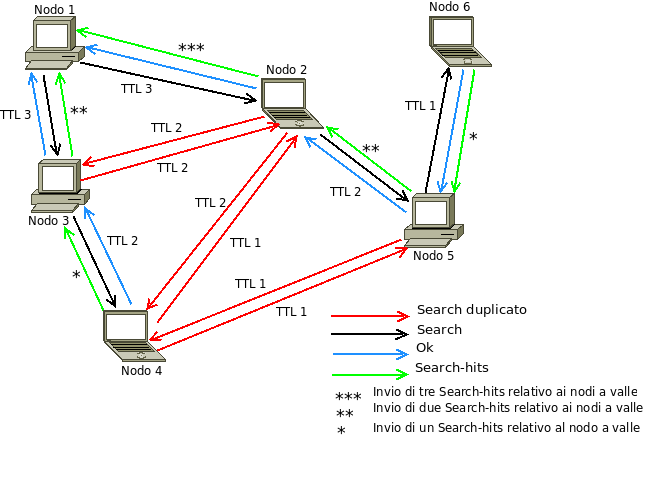
\includegraphics[scale=0.3]{etc/Search_overlay.png}
					\end{center}
				\end{figure}
			\end{frame}
		\subsection{Join e Leave}
			\begin{frame}
				\frametitle{Join}
				\begin{itemize}
					\item Il Join viene inviato a tutti i vicini.
					\item Evita inconsistenza dei dati.
					\item Diminuisce la probabilità di ricerca nulla.
					\item Tutti gli utenti connessi alla chat aggiungeranno l'utente.
				\end{itemize}
				\begin{figure}[H]
					\begin{center}
						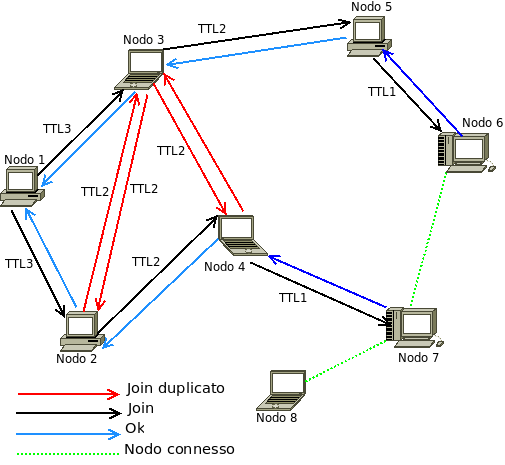
\includegraphics[scale=0.2]{etc/Join.png}
					\end{center}
				\end{figure}
			\end{frame}
			\begin{frame}
				\frametitle{Leave}
				\begin{itemize}
					\item Anche il Leave viene inviato a tutti i vicini.
					\item Tutti devono sapere che un peer sta lasciando la chat.
					\item Evita di inviare risultati errati dopo una ricerca.
				\end{itemize}
			\end{frame}
	
\end{document}

